\documentclass[a4paper,onecolumn]{extarticle}
\usepackage{geometry}
\usepackage[page,toc,titletoc,title]{appendix}
\usepackage{url}
\usepackage{caption}
\usepackage{subfigure}
\usepackage{subcaption}
\usepackage[sc]{mathpazo} % Use the Palatino font
\usepackage[T1]{fontenc} % Use 8-bit encoding that has 256 glyphs
\usepackage[utf8]{inputenc} % Use utf-8 as encoding
\linespread{1.05} % Line spacing - Palatino needs more space between lines
\usepackage{microtype} % Slightly tweak font spacing for aesthetics
\usepackage[spanish, activeacute]{babel}
 \decimalpoint
% \usepackage[hmarginratio=1:1,top=32mm,columnsep=20pt]{geometry} % Document marginshttps://www.overleaf.com/project/60211b96f72a79d4c7515e93
% \usepackage[hang, small,labelfont=bf,up,textfont=it,up]{caption} % Custom captions under/above floats in tables or figures
\usepackage{verbatim} % comentarios
\usepackage{listings}
\usepackage{xcolor}
\usepackage{wrapfig}
\lstset{
    inputencoding=utf8,
    frame=single,
    basicstyle=\fontsize{7}{10}\selectfont\ttfamily,
    basicstyle=\ttfamily\small,
    keywordstyle=\color{blue}\bfseries,
    identifierstyle=\color{black},
    commentstyle=\color{gray}\itshape,
    stringstyle=\color{red},
    numbers=left,
    numberstyle=\tiny\color{gray},
    stepnumber=1,
    numbersep=10pt,
    showspaces=false,
    showstringspaces=false,
    breaklines=true,
    breakindent=0pt,
    breakatwhitespace=false,
    tabsize=2,
    captionpos=b,
    literate={á}{{\'a}}1
        {ã}{{\~a}}1
        {é}{{\'e}}1
        {ó}{{\'o}}1
        {í}{{\'i}}1
        {ñ}{{\~n}}1
        {¡}{{!`}}1
        {¿}{{?`}}1
        {ú}{{\'u}}1
        {Í}{{\'I}}1
        {Ó}{{\'O}}1
}
\setlength{\parskip}{0.8em}
\usepackage{natbib}
\usepackage{enumitem}
% \setlist[itemize]{noitemsep} % Make itemize lists more compact
% \usepackage{abstract} % Allows abstract customization
% \renewcommand{\abstractnamefont}{\normalfont\bfseries} % Set the "Abstract" text to bold
% \renewcommand{\abstracttextfont}{\normalfont\small\itshape} % Set the abstract itself to small italic text
\usepackage{titlesec}

\usepackage{fancyhdr} % Headers and footers
\pagestyle{fancy} % All pages have headers and footers
\fancyhead{}
\lhead{Hugo Gómez Sabucedo}
\rhead{Minería de datos y modelización predictiva}

\renewcommand{\footrulewidth}{0.2pt}
\usepackage{titling} % Customizing the title section
\usepackage[breaklinks=true]{hyperref} % For hyperlinks in the PDF
%\usepackage{array}
%\newcolumntype{C}[1]{>{\centering\let\newline\\\arraybackslash\hspace{0pt}}m{#1}}
\usepackage{graphicx}
%\usepackage{lipsum} % NO NECESARIO LUEGO
%\usepackage{amsmath}
%\usepackage{wrapfig}
%\usepackage{multicol}
%\usepackage{bm}


\let\stdsection\section
\renewcommand\section{\newpage\stdsection}

%-------------------------------------------------------------------------------
%	TITLE SECTION
%-------------------------------------------------------------------------------

\setlength{\droptitle}{-4\baselineskip} % Move the title up



\title{\begin{center} \Huge Machine Learning: clasificación binaria\end{center}} % Article title
\author{
    \textsc{\Huge Hugo Gómez Sabucedo} \\ % Your name
    \large \href{mailto:hugogomezsabucedo@gmail.com}{hugogomezsabucedo@gmail.com} \\ [2ex] % Your email address
    \Large \textbf{Máster Big Data, Data Science \& Inteligencia Artificial} \\
    \normalsize Curso 2024-2025 \\
    \large Universidad Complutense de Madrid
}
\date{} % Leave empty to omit a date

\begin{document}
% Print the title
\maketitle
%\newpage
\tableofcontents
%\newpage
\begin{sloppypar}

%-------------------------------------------------------------------------
%	DOCUMENT
%-------------------------------------------------------------------------

\section{Introducción y análisis inicial} \label{introduccion}
En este trabajo, se nos proporciona un archivo con datos de ventas de coches de segunda mano, en el que se recogen diferentes características de los mismos, 
provenientes de una empresa de coches de segunda mano que debe determinar el color óptimo con el que repintar algunos vehículos que han llegado en un estado 
deficiente. El objetivo es realizar, para la empresa que nos proporciona los datos, un modelo predictivo que, en base a las características y variables, determine
si el vehículo debe pintarse de blanco o no.

Las características que se recogen para los vehículos son: el precio, el Levy o impuesto, el fabricante, el año de producción, la categoría, si el interior es 
o no de cuero, el tipo de combustible, el volumen del motor, el kilometraje, el número de cilindros, el tipo de caja de cambios, la tracción, el lado en donde 
se encuentra el volante y el número de airbags. Estas serán las variables predictoras que empleemos en nuestro modelo. Además, evidentemente, tenemos la variable 
color, que nos indica si el coche se pinta de blanco o negro, que será la variable que nos interese predecir.

\subsection{Análisis de los datos. Feature engineering}
En primer lugar, cargaremos el archivo en pandas, y el primer análisis que realizamos es ver la forma del dataframe y las cinco primeras columnas. Vemos que 
tenemos un dataframe con 15 columnas, tantas como variables habíamos comentado, y 4340 filas, y analizamos algunas de ellas para tener una idea de como son 
los datos y qué pasos podríamos seguir. El siguiente paso será ver si hay valores duplicados, y en este caso vemos que tenemos un total de 1534 valores duplicados.
Es una gran proporción de los datos, en torno a un 35\% de los mismos, aunque en este caso se ha optado por eliminarlos. Es una decisión drástica, ya que suponen 
una gran parte de los datos, pero se ha tomado debido a que se considera que lo que pueden aportar al modelo es menos de lo que lo entorpecen. Hay que tener en 
cuenta que, si se detectan como duplicados, es que tienen el mismo valor en exactamente todas las variables (precio, kilometraje, Levy, etc.), lo cual de por sí
ya es una situación difícil de encontrar. Esto ya no sólo aporta información redundante, y que podría alterar las estadísticas, sino que podría causar problemas 
de sesgo en el modelo resultante. Nuestro modelo se entrenará buscando patrones. Por tanto, la presencia de datos duplicados hará que ese patrón aparezca varias 
veces, lo cual hará que el modelo se sobreajuste a ello, produciéndose lo que se conoce como \textit{overfitting}. Por tanto, se decide eliminar todos los 
duplicados, para prevenir este problema.

\begin{wrapfigure}[10]{l}{3.75cm}
    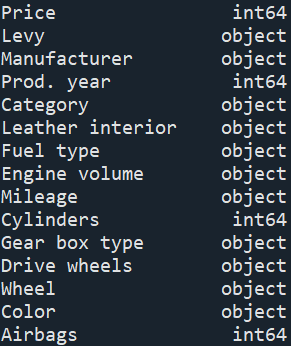
\includegraphics[width=0.25\textwidth]{imgs/dtypes.png}
    \caption{dtypes de las columnas} \label{fig:dtypes}
\end{wrapfigure}
A continuación, vemos los tipos que se han asignado a las diferentes columnas. Vemos que únicamente se asignan como numéricas el precio, año de producción, cilindros 
e airbags. De momento, no haremos ninguna corrección, ya que realizaremos posteriormente algunas transformaciones sobre las columnas que modificarán su tipo. 

\begin{figure}[h]
    \centering
    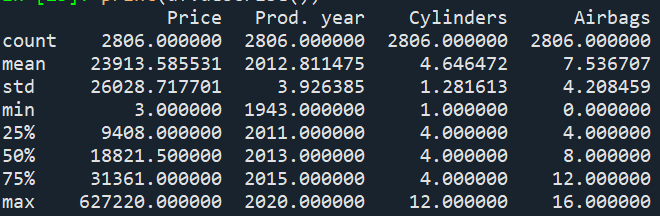
\includegraphics[width=0.5\textwidth]{imgs/describe inicial.png}
    \caption{Describe inicial} \label{fig:descInicial}
\end{figure}
Hacemos un describe inicial, para las variables que ha determinado como numéricas, donde vemos que el precio quizás tiene una ligera asimetría positiva, ya que 
su media es de 23.913 y su mediana de 18.821, inclinada un poco hacia valores más altos. Además, el máximo es muy superior al cuartil 75 (627.220 frente a 31.361). 
Además, la desviación típica es relativamente elevada, de 26.028, lo cual nos indica que claramente la variable está distribuida de forma asimétrica. Posteriormente,
trataremos este caso. Si hacemos un conteo de los valores missing, con un isnull y un isnan, vemos que no hay ninguna variable con valores faltantes, lo cual 
simplificará posteriormente el proceso.

\begin{wrapfigure}[20]{l}{4cm}
    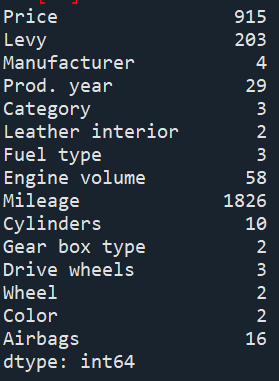
\includegraphics[width=0.28\textwidth]{imgs/nunique.png}
    \caption{Valores únicos en las columnas} \label{fig:nunique}
\end{wrapfigure}
El siguiente paso es analizar los valores únicos que hay en las columnas, para ver si, para las variables categóricas, podemos modificar o reagrupar algunas.
En este caso, vemos que hay variables con pocos valores únicos. Únicamente hay dos en \textit{Leather interior}, \textit{Gear box type}, \textit{Wheel} y, como 
es de esperar, en \textit{Color}; con tres, tenemos \textit{Category}, \textit{Fuel type} y \textit{Drive wheels}; y con cuatro, únicamente \textit{Manufacturer}.
En el caso de las que únicamente tienen dos valores, realizaremos una conversión o mapeo binario. En el caso de \textit{Leather interior}, mapearemos el Sí como 
un 1 y el No como un 0. Para \textit{Color}, White será un 1 y Black un 0. Para \textit{Wheel}, mapearemos `Right-hand drive` a 1 y `Left wheel` a 0, y renombraremos 
la columna como \textit{Right wheel}; para \textit{Gear box type}, mapearemos `Automatic` a 1 y `Triptonic` a 0, y renombraremos la columna a \textit{Automatic}.

A continuación, modificaremos la variable \textit{Engine volume}, para cambiar también su tipo. Se ha visto que, para algunos casos, la variable incluye el texto 
\textit{Turbo}, por lo que se decide emplear un \texttt{str.contains()} para detectar aquellas filas en las que esto ocurre. Esto se llevará a una nueva columna, 
llamada Turbo, que nos indique si efectivamente el motor es Turbo o no. Ya que es una variable binaria, la mapearemos como 1 en caso de que lo sea, y 0 en caso
de que no. Así, la variable \textit{Engine volume} quedará como una variable numérica, conteniendo solo el volumen del motor.

Siguiendo con la limpieza, se corrije la variable \textit{Mileage} para que pase a ser numérica, eliminando el texto `km` que contenía el mismo, y convirtiéndola 
a entera. Respecto a la variable \textit{Levy}, se ha visto que tiene el valor `-` en muchos casos, que podría indicar que ese coche en cuestión no tiene impuesto. 
En este caso, se ha decidido imputar este valor como un 0, manteniendo el valor original que hubiera en el resto de los casos. Esto nos permitirá tratar también 
esta variable como numérica, que es efectivamente el tipo de datos que debería tener. 

Con todo esto, podemos definir nuestras variables numéricas y categóricas, que quedan de la siguiente forma:
\begin{lstlisting}[language=Python,numbers=none]
nums = ['Price', 'Prod. year', 'Leather interior', 'Engine volume', 'Mileage', 'Airbags', 'Cylinders', 'Right wheel', 'Automatic', 'Turbo', 'Levy']
cats = ['Manufacturer', 'Category', 'Fuel type', 'Drive wheels']
target = "Color"
\end{lstlisting}

A continuación, analizaremos las variables categóricas, viendo la distribución de las categorías, para ver si es necesario reclasificar. En el caso de la variable 
\textit{Manufacturer}, tenemos un 37\% de coches de Hyundai, un 36,4\% de Toyota, un 18,4\% de Mercedes y un 8,2\% de Lexus. Esta última categoría podría estar 
poco representada, pero se ha decidido no hacer una reagrupación ya que puede resultar interesante dejar los datos como están. Además, la decisión lógica sería 
agruparla con los coches de Mercedes, lo cual no tiene mucho sentido, al tratarse de una marca de gama superior, para la cual es esperable que los coches, aún 
siendo de segunda mano, tengan un valor económico superior.

En el caso de \textit{Category}, tenemos un 52,7\% de coches sedán, un 23\% de jeep y un 14,6\% de hatchback. En este caso, no hay ninguna categoría que 
tenga menos de un 10\% de los valores, por lo que no es necesario reagrupar. Las categorías no están distribuidas uniformemente, pero es algo que puede ser normal.
En el caso de \textit{Fuel type}, un 55,5\% de coches son de gasolina, un 23\% son híbridos y un 21,5\% son diésel. De nuevo, ninguna categoría es inferior al 
10\%. Vemos que la mayoría de los coches son de gasolina pero, teniendo en cuenta que son datos de EEUU, donde este tipo de coches es el habitual, no parece raro.

Por último, tenemos \textit{Drive wheels}, donde vemos que un abrumador 71,6\% tiene tracción delantera, un 18,4\% es 4x4 y un 9,9\% es de tracción trasera. En 
este caso, si que se hace una reagrupación, ya que claramente hay una categoría predominante. Se ha decidido agrupar los vehículos de 4x4 con los de tracción 
trasera. Esta reagrupación nos dejaría, además, una variable binaria, por lo que la renombramos como \textit{Front drive}, donde un 1 significará la tracción 
delantera, mientras que un 0 significará que no tiene tracción delantera (bien sea porque es 4x4 o porque es de tracción trasera).

\begin{figure}[h]
    \centering
    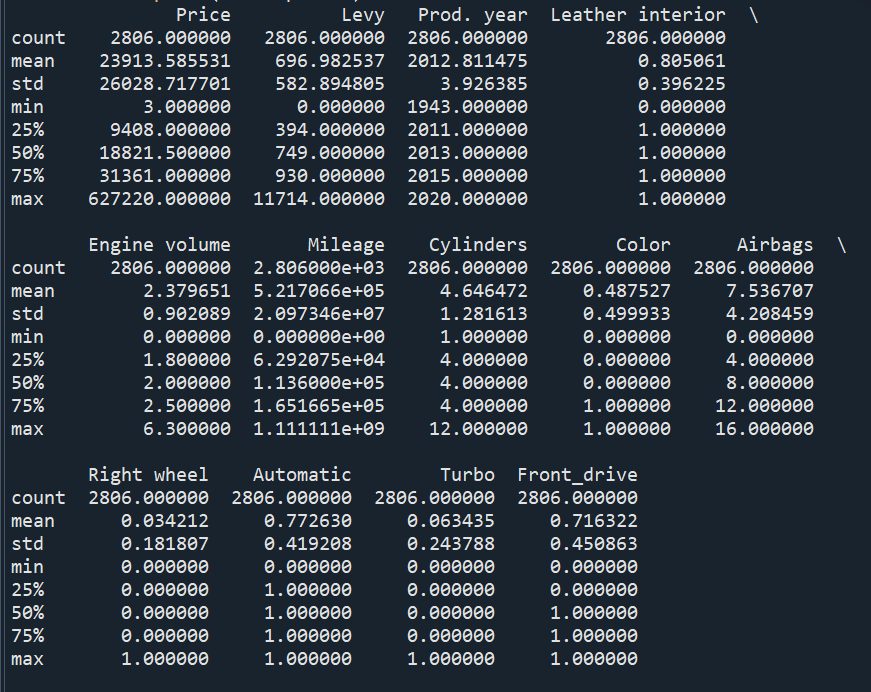
\includegraphics[width=0.5\textwidth]{imgs/descriptivos.png}
    \caption{Descriptivos} \label{fig:descriptivos}
\end{figure}
El siguiente paso es la búsqueda de outliers. En la imagen \ref{fig:descriptivos} se pueden ver los descriptivos de cada una de las variables numéricas, que
ahora son más que las analizadas inicialmente. Algunos casos destacables que vemos es el precio, con un máximo relativamente alto. Sin embargo, para esta variable,
hemos decidido no hacer ninguna imputación, ya que se entiende que un precio muy elevado podría tratarse de algún vehículo histórico, o con algunas características 
especiales o únicas, que justificaran este precio. El año de producción tiene dos valores claramente atípicos, ya que el mínimo es de 1943, mientras que vemos que 
el resto de años son en torno a la década de los 90. Además, en la figura \ref{fig:boxplot}, vemos que en 1986 tenemos otro valor atípico. Los eliminaremos 
directamente ya que se trata únicamente de dos registros. Se ven también unos cuantos datos que podrían ser atípicos en la década de los 90, pero hemos decidido 
dejarlos, ya que consideramos que pueden aportar al modelo tener unos coches un poco más ''antiguos''.
\begin{figure}[h]
    \centering
    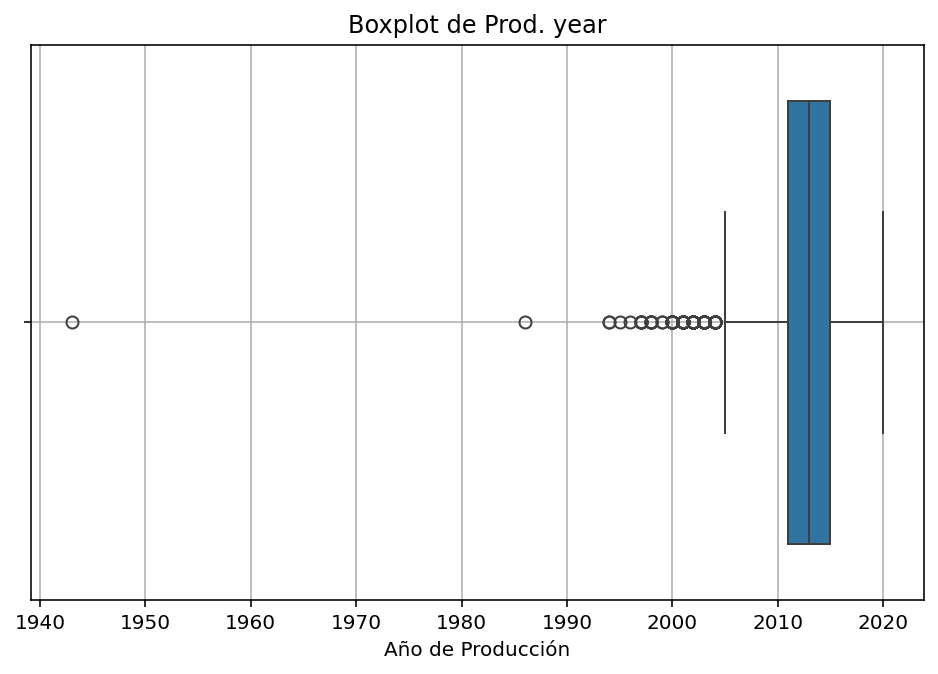
\includegraphics[width=0.5\textwidth]{imgs/boxplot.png}
    \caption{Boxplot de año de producción} \label{fig:boxplot}
\end{figure}

Respecto a \textit{Engine volume}, tenemos un mínimo de 0, un valor que se repite en dos registros. Esta variable se refiere a la cilindrada del coche, que en 
ningún caso puede ser 0. Que se trate de dos valores indica claramente que es un error, por lo que eliminamos directamente estos registros. También vemos un 
valor mínimo de 0 en \textit{Airbags}, que aunque inicialmente puede parecer un error, puede tener sentido si los coches fueran muy antiguos, ya que estos se 
hacían en algunos casos sin airbags. No haremos nada en este caso. Por último, se ve que la variable de \textit{Levy} y \textit{Mileage} tienen máximos muy 
elevados, por lo que analizaremos más a fondo los valores atípicos. Para ello, hemos creado la siguiente función, que toma en cuenta el rango intercuartílico 
para discrimar qué valores son atípicos.
\begin{lstlisting}[language=Python]
def detect_outliers(df, column):
    Q1 = df[column].quantile(0.25)
    Q3 = df[column].quantile(0.75)
    IQR = Q3 - Q1
    lower_bound = Q1 - 1.5 * IQR
    upper_bound = Q3 + 1.5 * IQR
    return df[(df[column] < lower_bound) | (df[column] > upper_bound)]
\end{lstlisting}

Esto nos da un total de 92 outliers en la primera variable y un total de 81 en la segunda variable. Estos datos, un total de 173 valores atípicos (que podrían 
ser incluso menos, ya que puede que haya una fila que sea atípica en ambas variables) representa apenas un 4\% de los datos, por lo que, en lugar de perder 
tiempo en la imputación de los valores atípicos, se ha decidido optar por eliminarlos directamente. Con esto, ya tenemos todas las variables limpias, así que 
podemos pasar a convertir las variables categóricas a dummies, que es uno de los requisitos que hay para poder aplicar los modelos.

\begin{figure}[h]
    \centering
    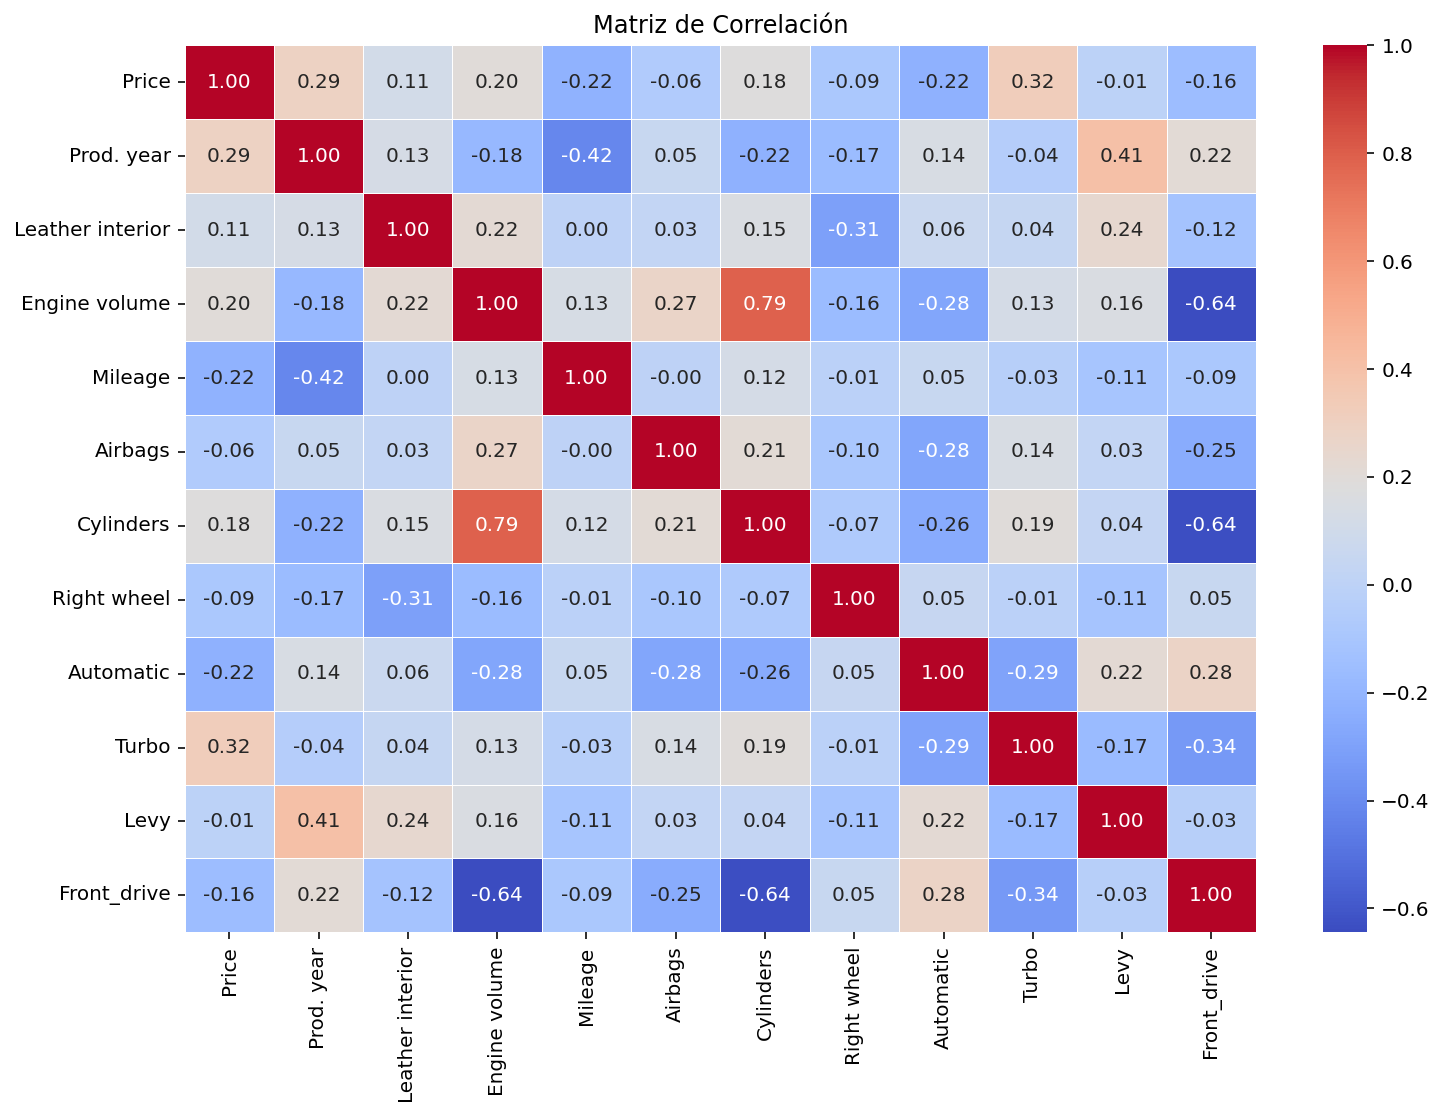
\includegraphics[width=0.6\textwidth]{imgs/correlacion.png}
    \caption{Matriz de correlación de las variables} \label{fig:correlacion}
\end{figure}
Una vez creadas las variables dummies, analizamos la correlación que hay entre las variables, para ver si es necesario eliminar alguna de ellas. En la imagen 
\ref{fig:correlacion} tenemos dicha matriz de correlación, en la cual vemos dos cosas que destacan. Por una parte, \textit{Front drive} tiene una correlación 
de -0,64 (es decir, negativa) tanto con \textit{Engine volume} como con \textit{Cylinders}, lo cual es esperable ya que suelen ser motores más compactos; por 
otra parte, una elevada correlación positiva entre los cilindros y el \textit{Engine volume}, de 0,79, lo cual tiene sentido ya que un motor con más cilindros
tiende a tener más \textit{Engine volume}. En este caso, ya que se dice que es adecuado eliminar las variables con una correlación superior a 0,8 (tanto negativa
como positiva), eliminaremos la variable de \textit{Cylinders}. Dejaremos las otras dos, ya que un 0,64 de correlación no se acerca al umbral indicado como 
para eliminarlas.

Por último, separamos el dataframe en las variables predictoras o independientes y la variable que queremos predecir, y dividimos los datos en entrenamiento y 
prueba, con un tamaño de prueba del 30\%. A continuación, realizamos una estandarización de los datos. Esto se hace ya que los algoritmos que emplearemos, como 
es el SVM, es bastante sensible a la escala de los datos, y un rango muy grande en una variable podría hacer que esta sobredomine el modelo. Con esto, ya tenemos
los datos listos con los que aplicar el modelo.

\section{Modelo de SVM}\label{SVM}
\subsection{Ajuste del modelo}\label{ajuste}
Para crear y ajustar los modelos, aplicaremos un grid search para probar diferentes parámetros con los tres kernels que se han elegido, que en este caso son el 
linear, el polinómico y el gaussiano o rbf. El grid search tiene varias ventajas, pero la principal es que nos evita tener que probar uno a uno todos los 
posibles valores de los parámetros para encontrar el óptimo. Él los probará todos, y nos devolverá la combinación que nos devuelva el mejor resultado. De esta 
forma, nosotros sólo tendremos que elegir con qué kernel nos quedamos. Además, el propio \texttt{GridSearchCV} usa validación cruzada, lo cual evita también 
un sobreajuste del modelo a una partición concreta de los datos. Por lo tanto, esta es la mejor opción para poder explorar distintos parámetros, y ver con cuál
obtenemos el mejor de los resultados. En este caso, para cada uno de los kernels, se definen los siguientes parámetros:
\begin{lstlisting}[language=Python,]
    param_grid_linear = {'C': [0.1, 0.5, 1, 2, 5, 10, 100]}
    param_grid_poly = {'C': [0.1, 0.5, 1, 2, 5, 10, 100], 'degree': [2, 3, 4], 'coef0': [0, 1, 2]}
    param_grid_rbf = {'C': [0.1, 0.5, 1, 2, 5, 10, 100], 'gamma': [0.1, 0.5, 1, 2, 5]}
\end{lstlisting}

En este caso, el parámetro C es común a todos los kernels, y es el parámetro de penalización, que controla el equilibro entre tener un margen amplio y clasificar 
bien los datos. Un C pequeño da más margen, pero con más errores; un C alto penalizará más los errores, pero podría llevar también a overfitting. Este es el 
único parámetro que se usa en el kernel linear. En el polinómico se añaden dos más: por una parte, degree, que indica el grado del polinomio que se usa para 
crear la función de decisión, que será más compleja cuanto mayor sea el valor. En este caso, se usarán términos cuadráticos, cúbicos y a la cuarta potencia; y 
por otra parte, coef0, que es el término independiente que se sumará al polinómico, que ayuda a ajustar la flexibilidad del modelo. Para el kernel gaussiano, 
tenemos un único parámetro adicional que es gamma, y que controla la influencia de cada ejemplo: un gamma bajo significa que los puntos lejanos también influyen, 
lo que nos da un modelo más suave; mientras que un gamma alto hace que sólo influyan los puntos más cercanos, dando un modelo más complejo pero con riesgo de que 
se produzca overfitting. 

Una vez hecho el grid search, obtenemos el mejor parámetro para cada uno de los kernel. En el caso del linear, el mejor parámetro es un C=0,1. Para el kernel 
polinómico, el mejor parámetro es un C=0,1, un degree=2 y un coef0=2. Para el kernel gaussiano, los mejores parámetros son C=2 y un gamma=0,5. Como podemos ver,
los mejores modelos son modelos sencillos, con un parámetro C que penaliza poco los errores (por lo que no estamos arriesgando en overfitting), y polinomios 
sencillos. Hacemos las predicciones con cada uno de los mejores modelos para cada uno de los kernel, y mostramos el reporte de clasificación de los resultados 
que nos da la función \texttt{classification\_report}, como se ve en la imagen \ref{fig:reportKernels}. Aquí vemos que los tres modelos tienen accuracy muy
similar, y que aunque el resultado está redondeado a dos decimales, en realidad es prácticamente la misma: 0,627 para el linear, claramente la ''menor'' de todas;
0,641 para el polinómico y 0,645 para el gaussiano.
\begin{figure}[h]
    \centering
    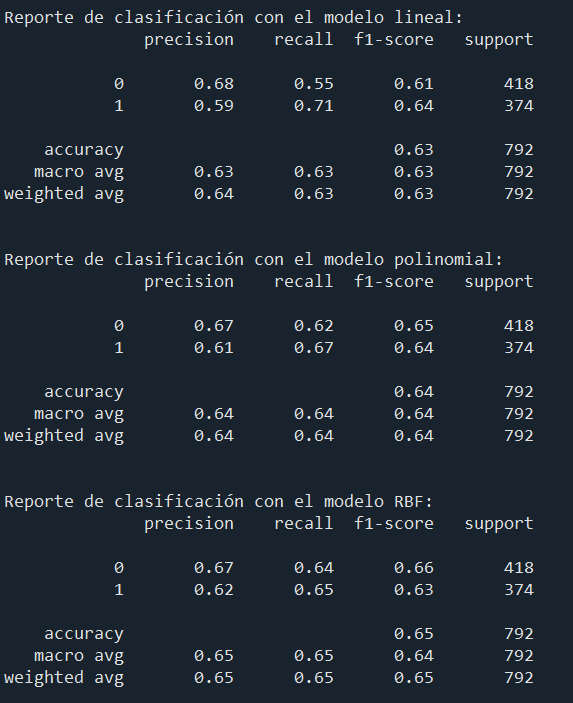
\includegraphics[width=0.5\textwidth]{imgs/reportKernels.png}
    \caption{\textit{Classification report} para SVM} \label{fig:reportKernels}
\end{figure}

Mostramos también cada una de las tres matrices de confusión, que se ven en \ref{fig:confusiones}. La matriz de confusión representa [[TP, FP], [FN, TN]]. TP son 
los verdaderos positivos, los datos que se clasificaron correctamente como positivos; FP los falsos positivos, los que se clasificaron como positivos (en este caso,
white), pero eran negativos (eran black); FN los falsos negativos, los que se clasificaron como negativos pero eran positivos; y TN los verdaderos negativos, los 
que se clasificaron correctamente como negativos. El modelo lineal tiene un numero elevado de falsos positivos, pero tambien una gran proporción de verdaderos 
positivos y negativos. Podría mejorar en la clasificación de la clase black, pero es bastante efectivo. El polinómico mejora los falsos positivos, aunque a costa 
de empeorar ligeramente los falsos negativos, pero sigue teniendo un buen rendimiento. El gaussiano, por último, es el que menos falsos positivos tiene, pero 
mejora a costa de empeorar los falsos negativos, como en el caso anterior, y es también el que más falsos negativos tiene. Aún así, en general, el polinómico 
parece ser el que está más equilibrado.
\begin{figure}[h!]
    \centering
    \begin{minipage}[b]{0.3\textwidth}
        \centering
        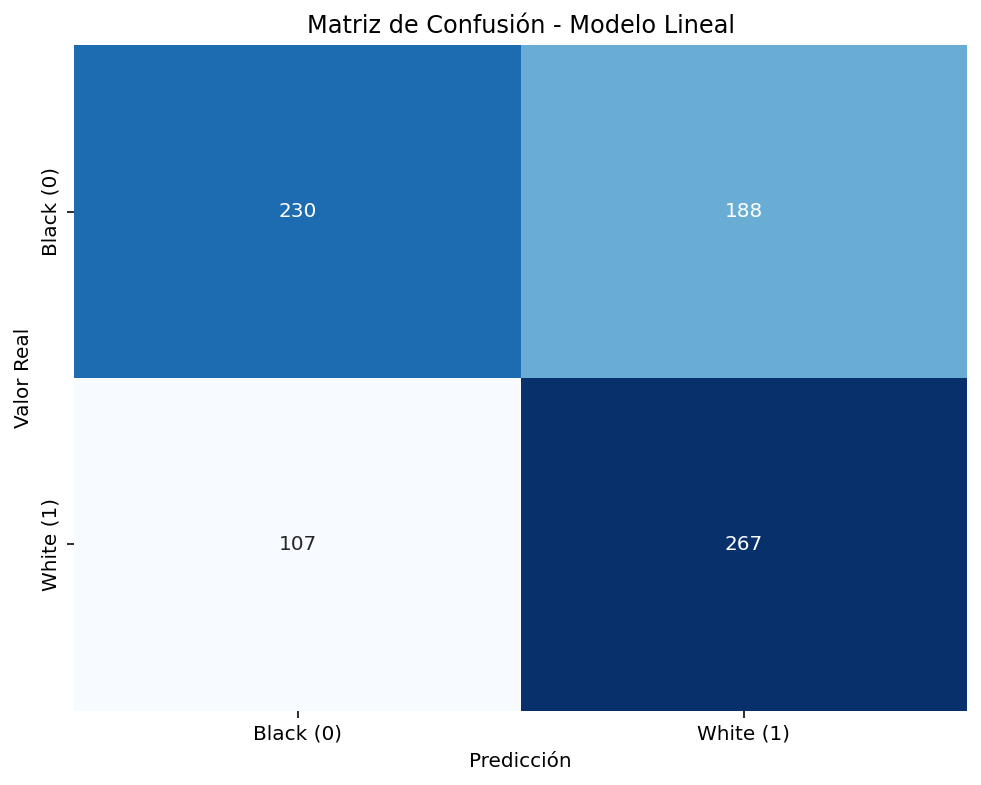
\includegraphics[width=\textwidth]{imgs/confLin.png}
        \caption{Kernel linear}
    \end{minipage}%
    \hspace{1em}  % Espacio entre las imágenes
    \begin{minipage}[b]{0.3\textwidth}
        \centering
        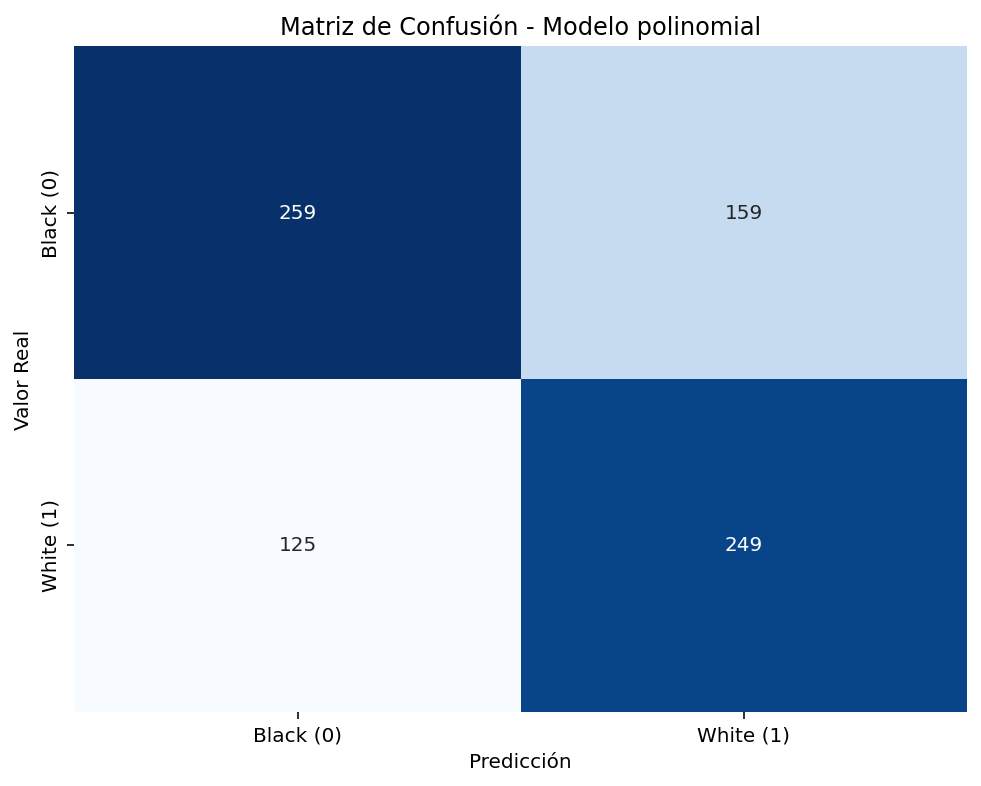
\includegraphics[width=\textwidth]{imgs/confPol.png}
        \caption{Kernel polinómico}
    \end{minipage}%
    \hspace{1em}  % Espacio entre las imágenes
    \begin{minipage}[b]{0.3\textwidth}
        \centering
        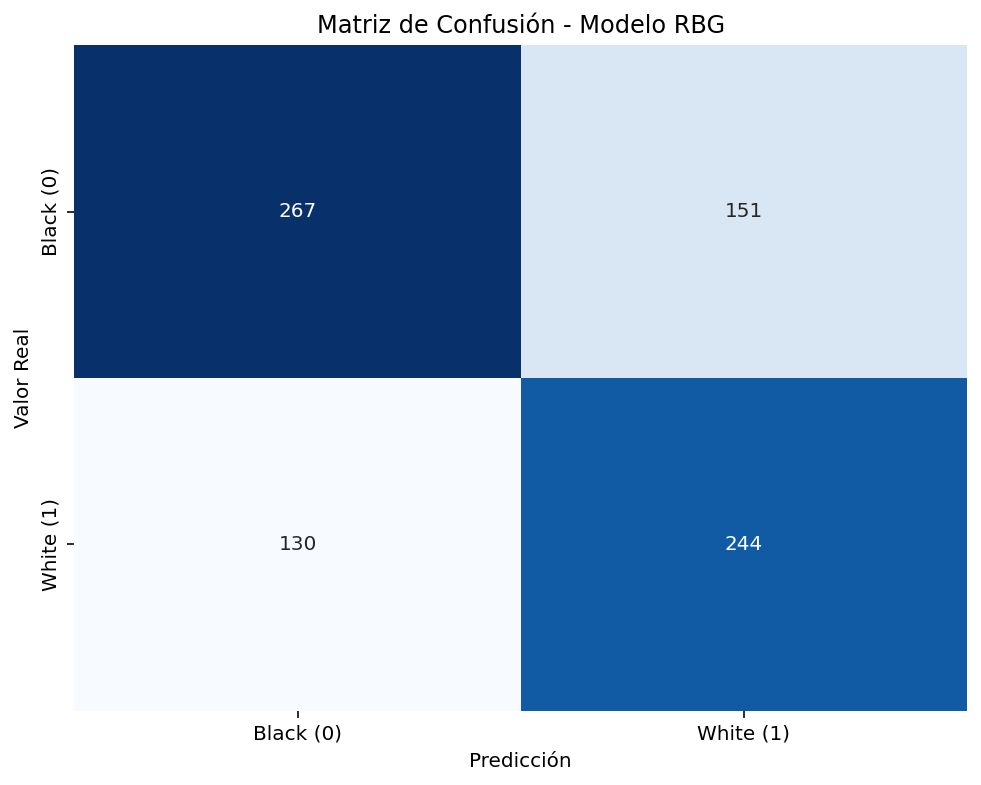
\includegraphics[width=\textwidth]{imgs/confGaus.png}
        \caption{Kernel gaussiano}
    \end{minipage}
    \label{fig:confusiones}
\end{figure}

Además, mostramos también el área bajo la curva ROC, que en este caso se ha decidido hacer de forma conjunta para los tres modelos, como se ve en la imagen 
\ref{fig:AUC}. Esto nos sirve para evaluar también el rendimiento del modelo, ya que muestra la relación entre FP y TP. Un valor próximo a 1 indica un rendimiento 
perfecto, mientras que menor que 0,5 indica que es peor que el azar, que clasifica al revés y mal. En este caso, el mejor valor del AUC se da en el polinómico, 
con un AUC de 0,7038, mientras que el más bajo es el 0,6708 del gaussiano, estando el lineal con 0,6971 entre medias.
\begin{figure}[h]
    \centering
    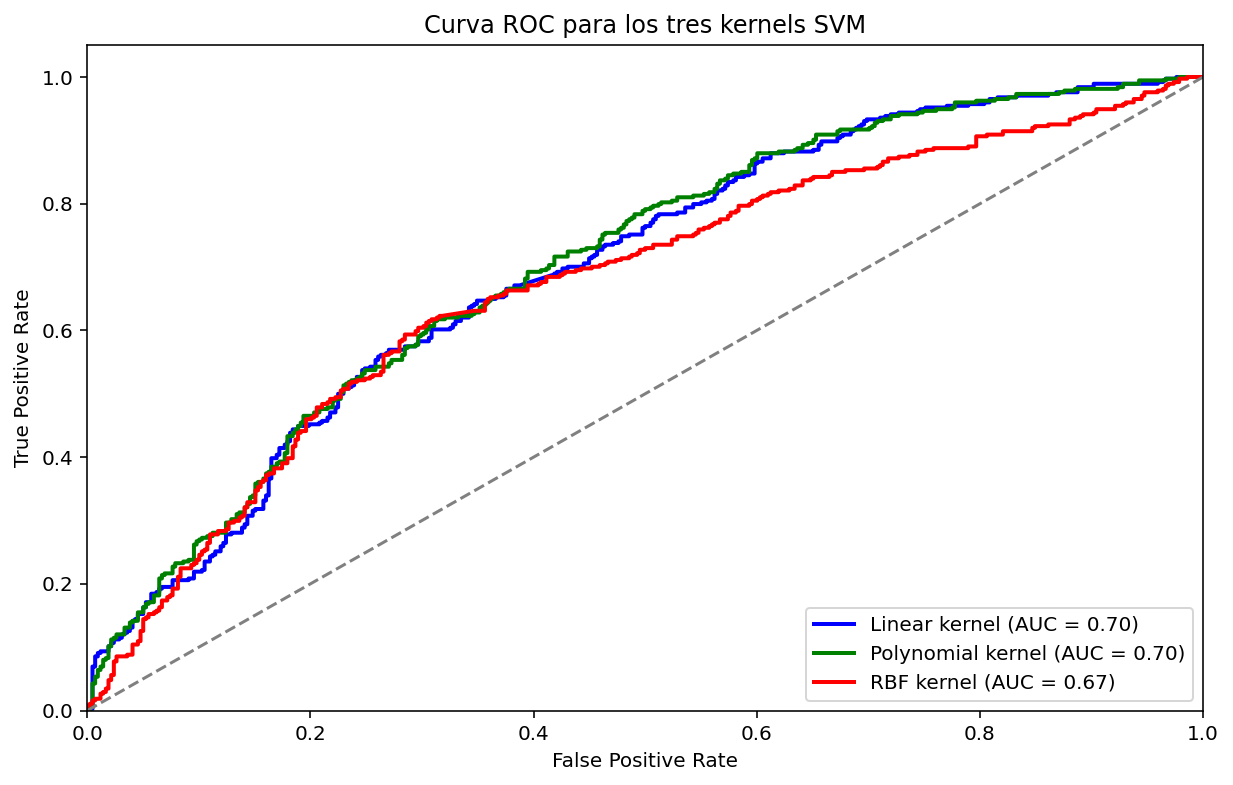
\includegraphics[width=0.6\textwidth]{imgs/curvaROC.png}
    \caption{Área bajo la curva ROC} \label{fig:AUC}
\end{figure}

Para elegir el mejor modelo empleamos estos tres indicadores: las matrices de confusión, la \textit{accuracy} y el área bajo la curva ROC. Aunque el kernel
gaussiano es el que tiene mejor precisión, como comentamos, todos los valores son prácticamente iguales, por lo que debemos fijarnos en los demás indicadores. 
El polinómico tiene un AUC bastante más alto que el gaussiano, un 3\% más, con sólo un 0,4\% de diferencia en la precisión. Además, el AUC es una métrica que, 
en este caso, tratándose de un problema de clasificación, es más fiable o útil, ya que considera cómo de bien clasifica el modelo, y tiene en cuenta tanto la 
tasa de verdaderos positivos como la d efalsos positivos. Por lo tanto, se elige el polinómico como el mejor modelo, al que se le aplicará el bagging.

\subsection{Aplicación de bagging}\label{bagging}
El bagging, o bootstrap aggregating, es una técnica de ensamblaje de modelos que se suele usar para mejorar la estabilidad y precisión de modelos de aprendizaje
automático, especialmente en casos como el nuestro de clasificación, buscando reducir la varianza mediante la agregación de varios modelos. Además, permite mejorar
la generalización y evitar el overfitting, al usar las predicciones de varios modelos. Se suele aplicar para mejorar la predicción del modelo, reducir en la 
medida de lo posible el overfitting y acelerar el proceso de entrenamiento. En nuestro caso, empleamos el \texttt{BaggingClassifier} con el modelo que elegimos 
como mejor, con 50 estimadores como modelos base para entrenarlo, empleando un 70\% de los datos originales para el entrenamiento y seleccionando el 100\% de 
las características.
\begin{figure}[h!]
    \centering
    \begin{minipage}[b]{0.45\textwidth}
        \centering
        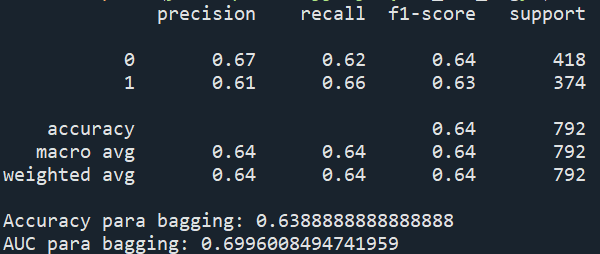
\includegraphics[width=\textwidth]{imgs/reportBagging.png}
        \caption{Classification report, accuracy y AUC para bagging}
        \label{fig:baggingACC}
    \end{minipage}%
    \hspace{1em}  % Espacio entre las imágenes
    \begin{minipage}[b]{0.45\textwidth}
        \centering
        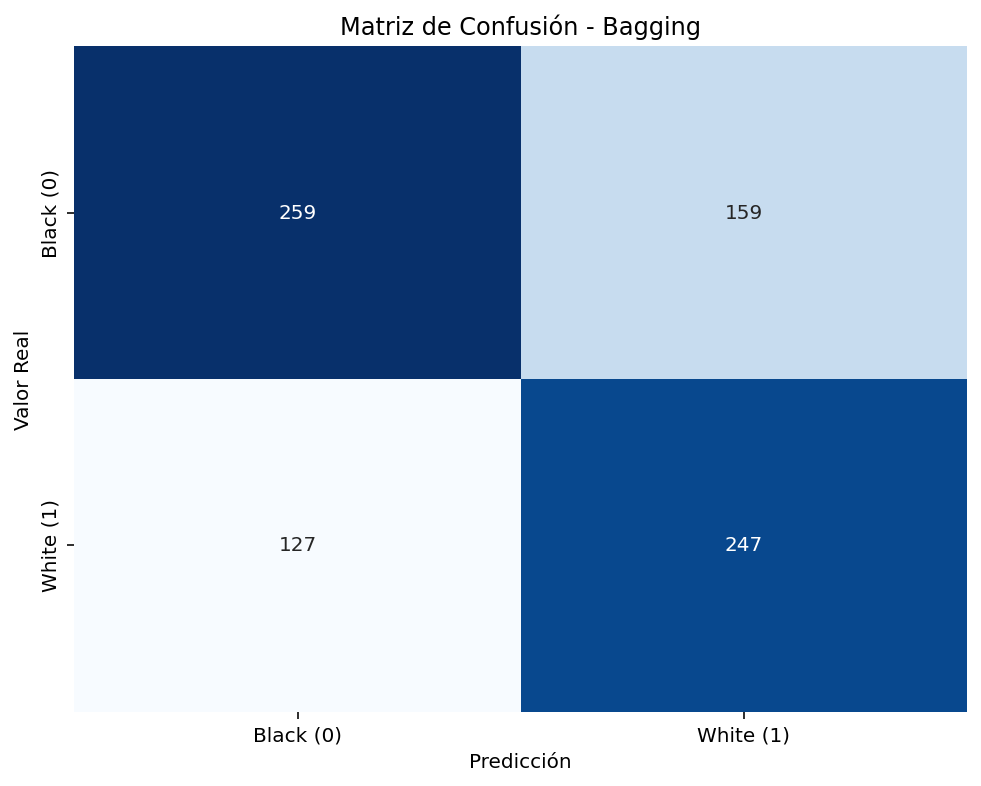
\includegraphics[width=\textwidth]{imgs/confBagging.png}
        \caption{Matriz de confusión para bagging}
        \label{fig:baggingConf}
    \end{minipage}
\end{figure}

Los resultados obtenidos para la matriz de confusión, precisión, AUC y el reporte de clasificación se ven en las figuras \ref{fig:baggingACC} y 
\ref{fig:baggingConf}, pero los comentaremos en la sección \ref{comparativa} para comparar entre el modelo sin y conn bagging, y los modelos obtenidos del 
stacking, que se trata en la siguiente sección.

\section{Modelo de stacking en profundidad}\label{stacking}
El stacking, es una técnica de ensamblaje que se basa en la combinación de distintos modelos, denominados modelos base, para crear un modelo final que sea más 
robusto y preciso, al realizar una combinación de los mismos. Para ello, se entrena una serie de modelos base sobre el mismo conjunto de datos, y luego se 
usa un metaclasificador que combine las predicciones de dichos modelos, con el objetivo de aprovechar las distintas virtudes de cada uno de los modelos.

En nuestro caso, hemos elegido tres modelos base: Random Forest, Logistic Regression y K-Neighbors.
\begin{itemize}
    \item \textbf{Random Forest} se basa en árboles de decisión, entrenando cada árbol con una muestra aleatoria de los datos. En cada nodo, el árbol seleccionará
    la mejor característica para dividir los datos, empleando un criterio concreto, y combina la predicción individual de cada uno de los árboles. Su principal 
    ventaja es su robustez y su versatilidad.
    \item \textbf{Logistic Regression} se usa principalmente para tareas de clasificación binaria, por lo que es un modelo que no podía faltar. Utiliza una función
    con la cual combina linealmente cada una de las características de entrada en una probabilidad, que representa la clase de salida, para la cual se establece
    un umbral al partir del cual se considera una clase u otra. Su principal ventaja es su simplicidad y eficiencia, así como que predice probabilidades, pero 
    no es adecuado si no hay relaciones lineales entre las variables.
    \item \textbf{K-Nearest Neighbors} (o \textbf{KNN}) se basa en instancias, clasificando una instancia en base a los k vecinos más cercanos a la misma. Este 
    modelo calcula las distancias entre la instancia o dato de prueba y los de entrenamiento para realizar una predicción, selecciona los k vecinos más cercanos 
    y predice la clase más común entre ellos. No realiza un entrenamiento explícito, sino que se ''guarda'' los datos de entrenamiento y va clasificando en función
    de ellos. Su principal ventaja es la facilidad que tiene para entenderlo, que no es paramétrico y que es ideal para captar patrones locales
\end{itemize}

Como metaclasificador, se ha elegido un RandomForestClassifier, que en general tiende a mejorar el rendimiento global, a la vez que resiste el overfitting (gracias 
a promediar varias predicciones), y es fácilmente integrable en el stacking. Los modelos se entrenan individualmente, y posteriormente se combinan con el metaclasificador,
empleando para ello la función \texttt{StackingClassifier}. Además, se aplica validación cruzada de 5 pliegues. En la figura \ref{fig:stackingGeneral} vemos los
resultados globales del stacking, y en la \ref{fig:stackingDetalle}, los resultados para cada uno de los modelos.
\begin{figure}[h!]
    \centering
    \begin{minipage}[c]{0.45\textwidth}
        \centering
        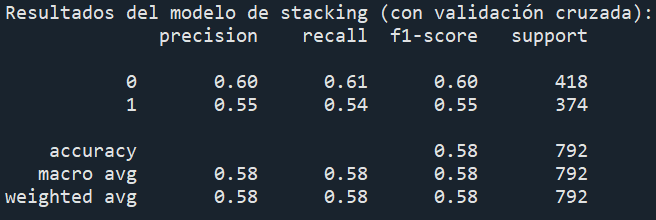
\includegraphics[width=\textwidth]{imgs/reportStacking.png}
        \caption{Resultados generales de stacking}
        \label{fig:stackingGeneral}
    \end{minipage}%
    \hspace{1em}  % Espacio entre las imágenes
    \begin{minipage}[c]{0.45\textwidth}
        \centering
        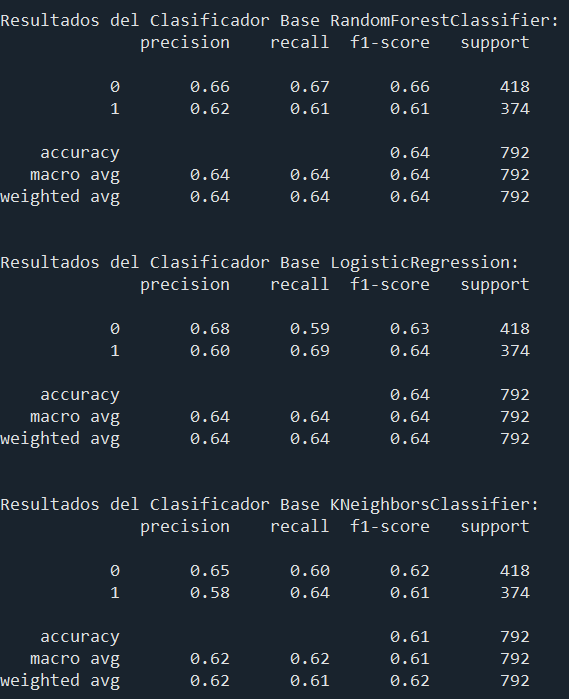
\includegraphics[width=\textwidth]{imgs/reportStackingModelos.png}
        \caption{Resultados de stacking modelo a modelo}
        \label{fig:stackingDetalle}
    \end{minipage}
\end{figure}

RandomForest obtuvo una precisión del 64, con un buen equilibrio entre precisión y recall. El LogisticRegression tiene una precisión similar, pero con un mejor 
equilibrio entre clases, con puntuación de 0,63 para la clase 0 y 0,64 para la 1. El KNeighbors es el que menor precisión tiene, con un 61\%, y por ende 
también una menor puntuación de f1. Al combinar los modelos con el metaclasificador, obtenemos una precisión del 58\%, con una puntuación de f1 para la clase 
0 de 0,60 y de 0,55 para la 1.

Es decir, el stacking no mejora los resultados. Esto puede deberse a que los modelos base ya obtenían resultados similares entre sí,
y no aportaban la diversidad suficiente como para que el metaclasificador los combine eficazmente. Además, puede que se haya cometido redundancia al usar como 
metaclasificador uno de los modelos base. Quizás probando con un metaclasificador más sencillo, como una regresión logística, empleando otro modelo base en su 
lugar, podríamos haber obtenido mejores resultados.

\section{Comparativa y conclusiones}\label{comparativa}
Una vez tenemos todos los modelos, los compararemos en base a, principalmente, la accuracy. En estos términos, el mejor modelo es el que escogimos como mejor 
del SVM, con un accuracy de 0,641, mejor incluso que aplicando bagging o stacking. Aunque la diferencia entre SVM y bagging es pequeña, la ventaja de SVM sugiere
que, en términos generales, este modelo tiene un mejor desempeño al clasificar correctamente las instancias en el conjunto de datos.

Esta comparativa en base a la accuracy no refleja por completo la calidad del modelo, pero no se ha podido realizar una comparativa más en profundidad. Lo que 
está claro es que, analizando todos los parámetros que hemos ido viendo para cada uno de los modelos, el mejor es el que resultó del SVM con un kernel polinómico.

\clearpage
%\newpage

%\appendix
%\section{Anexo: Código de la práctica}\label{anexo1}
%\lstinputlisting[language=Python]{codigoML.py}
\end{sloppypar}
\end{document}
